%\documentclass{beamer}
\documentclass[aspectratio=169]{beamer}
\usetheme{Boadilla}
%\usetheme{Warsaw}
%\setbeamercovered{transparent}
\beamertemplatetransparentcoveredhigh
\usepackage[portuges]{babel}
\usepackage[utf8]{inputenc}
\usepackage{lmodern}
\usepackage[T1]{fontenc}
\usepackage{hyperref} 
\usepackage{listings}
\usepackage{color}

\definecolor{dkgreen}{rgb}{0,0.6,0}
\definecolor{gray}{rgb}{0.5,0.5,0.5}
\definecolor{mauve}{rgb}{0.58,0,0.82}

\lstset{frame=tb,
  language=C,
  aboveskip=3mm,
  belowskip=3mm,
  showstringspaces=false,
  columns=flexible,
  basicstyle={\small\ttfamily},
  numbers=none,
  numberstyle=\tiny\color{gray},
  keywordstyle=\color{blue},
  commentstyle=\color{dkgreen},
  stringstyle=\color{mauve},
  breaklines=true,
  breakatwhitespace=true,
  tabsize=3
}
\title[Matrizes]{Matrizes\\
   Algoritmos e Estrutura de Dados I}
\author[IEng - UFMT]{Instituto de Engenharia -- UFMT}
%\institute[2020/2]{Segundo Semestre de 2020}
\date{}



\begin{document}

%------------------------------------------------
\begin{frame}[plain]
  \titlepage
\end{frame}

%------------------------------------------------

\begin{frame}
\frametitle{Roteiro} % Table of contents slide, comment this block out to remove it
\tableofcontents % Throughout your presentation, if you choose to use \section{} and \subsection{} commands, these will automatically be printed on this slide as an overview of your presentation
\end{frame}

%----------------------------------------------------------------------------------------
%	PRESENTATION SLIDES
%----------------------------------------------------------------------------------------

%------------------------------------------------
\section{Objetivos}

\begin{frame}
\frametitle{Objetivos}
Esta aula tem como objetivos:

\begin{enumerate}
\item Apresentar os conceitos básicos sobre Matrizes;
\item Explicitar os exemplos de funções que manipulam Matrizes;
\item Exemplificar a execução desses algoritmos.
\end{enumerate}
\end{frame}


%------------------------------------------------
\section{Introdução} % Sections can be created in order to organize your presentation into discrete blocks, all sections and subsections are automatically printed in the table of contents as an overview of the talk
%------------------------------------------------

\begin{frame}[fragile]
\frametitle{Introdução}
\begin{itemize}
\item Imaginemos que queremos ler as notas de 4 provas para cada aluno e calcular a média do aluno e a média da classe.
\item O tamanho máximo da turma é de 50 alunos.
\item Uma solução seria criar 4 vetores cada um com 50 posições e então ler as respectivas informações.
\end{itemize}
\begin{lstlisting}
 float nota1[50], nota2[50], nota3[50], nota4[50];
\end{lstlisting}
\end{frame}

%----------------------------------------------------------------------------------------

\begin{frame}
\frametitle{Introdução}
\begin{figure}[!h]
  \centering
  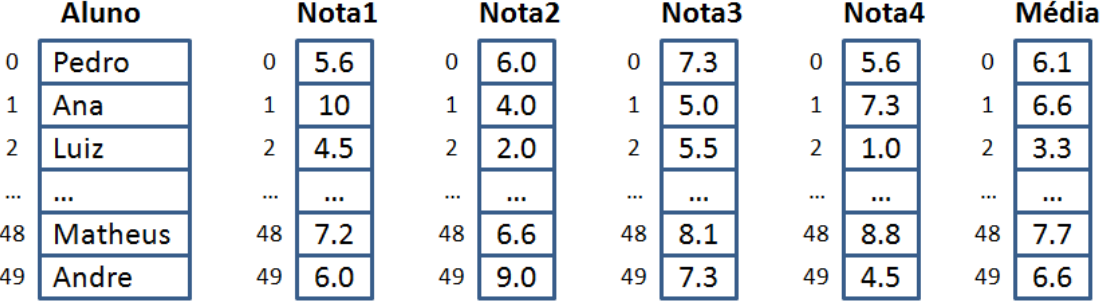
\includegraphics[width=300pt]{imgs/vetores.png}
  \label{fig_vetores}
\end{figure}
\end{frame}

%----------------------------------------------------------------------------------------

\begin{frame}
\frametitle{Introdução}
\begin{itemize}
\item Agora suponha que estamos trabalhando com no máximo 100 provas e 50 alunos.
\item Seria cansativo criar 100 vetores e atribuir 100 nomes diferentes.
\begin{figure}[!h]
  \centering
  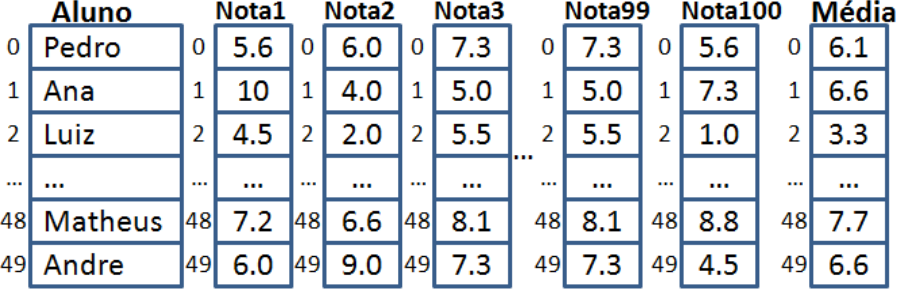
\includegraphics[width=200pt]{imgs/vetores2.png}
  \label{fig_vetores2}
\end{figure}
\item Para resolvermos esse problema, utilizamos matrizes.
\end{itemize}
\end{frame}

%----------------------------------------------------------------------------------------

\begin{frame}
\frametitle{Introdução}
\begin{itemize}
\item Uma matriz é um vetor (conjunto de variáveis de mesmo tipo) que possui duas ou mais dimensões.
\item Matrizes podem ser considerados como ``vetores de vetores''.
\item Por exemplo, uma matriz bidimensional pode ser vista como uma tabela de $m$ linhas e $n$ colunas.
\end{itemize}
\begin{figure}[!h]
  \centering
  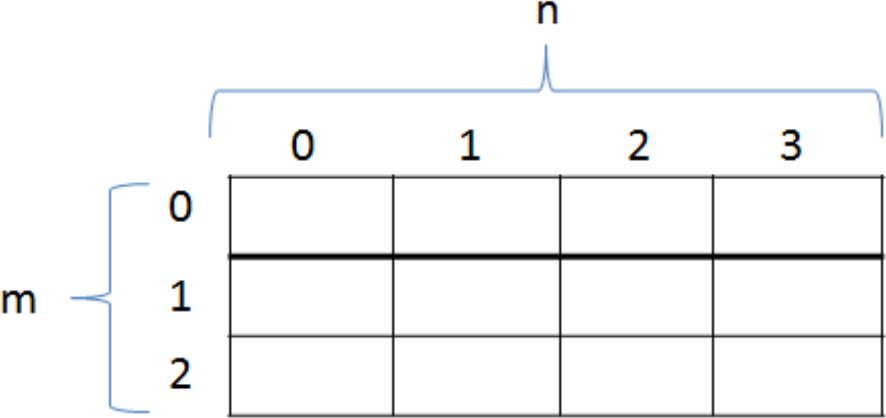
\includegraphics[width=200pt]{imgs/matrizes.png}
  \label{fig_matrizes}
\end{figure}
\end{frame}

%----------------------------------------------------------------------------------------

\section{Manipulando matrizes}

\begin{frame}[fragile]
\frametitle{Declarando uma matriz}
\begin{itemize}
\item Utiliza-se a forma geral para declaração de matrizes:
\begin{lstlisting}
 <tipo> nome_da_matriz [<linhas>][<colunas>];
\end{lstlisting}
\item Uma matriz possui linhas x colunas do tipo <tipo>.
\item As linhas são numeradas de 0 a linhas -1.
\item As colunas são numeradas de 0 a colunas -1.
\item Exemplo:
\end{itemize}
\begin{lstlisting}
 // Matriz com 100 linhas e 50 colunas
 float notas[100][50];
\end{lstlisting}
\end{frame}

%----------------------------------------------------------------------------------------

\begin{frame}[fragile]
\frametitle{Acessando elementos da matriz}
\begin{itemize}
\item Para acessar um elemento da matriz deve-se especificar a linha e coluna:
\begin{lstlisting}
 nome_da_matriz [<linha>][<coluna>];
\end{lstlisting}
\item Exemplo: imprimir o elemento da linha 1 e coluna 10.
\begin{lstlisting}
printf("%d", matriz[1][10]);
\end{lstlisting}
\item O compilador não verifica se foram utilizados valores válidos para a linha e para a coluna.
\end{itemize}
\end{frame}

%----------------------------------------------------------------------------------------

\begin{frame}[fragile]
\frametitle{Atribuindo valores para a matriz}
\begin{itemize}
\item Para atribuir um valor para um elemento da matriz deve-se especificar a linha e coluna:
\begin{lstlisting}
 nome_da_matriz [<linha>][<coluna>] = 0;
\end{lstlisting}
\item Para atribuir zero a todos os elementos da matriz é necessário um laço de repetição para cada dimensão da matriz. 
\item Por exemplo, para uma matriz bidimensional, são necessários dois laços de repetição:
\begin{lstlisting}
  int matriz[100][50], i,j;
  for(i=0;i<100;i++) {
    for(j=0;j<50;j++) {
      matriz[i][j] = 0;
    }
  }
\end{lstlisting}
\end{itemize}
\end{frame}

%----------------------------------------------------------------------------------------

\section{Exemplos}

\begin{frame}
\frametitle{Exemplo}
Criar uma matriz com 3 linhas e 4 colunas, inicializar a matriz com valores fornecidos pelo usuário e imprimir o valores.
\end{frame}

%----------------------------------------------------------------------------------------

\begin{frame}[fragile]
\frametitle{Exemplo}
\begin{lstlisting}
#include<stdio.h>
int main() {
  int matriz[3][4], i, j;
  // Inicializa a matriz com valores fornecidos pelo usuario
  for (i=0;i<3;i++) {
    for (j=0;j<4;j++) {
      scanf("%d",&matriz[i][j]);
    }
  }
  // Imprime a matriz
  for (i=0;i<3;i++) {
    for (j=0;j<4;j++) {
      printf("%d",matriz[i][j]);
    }
    printf("\n");
  }   
  return 0;
}
\end{lstlisting}

\end{frame}

%----------------------------------------------------------------------------------------

\begin{frame}
\Huge{\centerline{Dúvidas}}
\end{frame}

%----------------------------------------------------------------------------------------


\begin{frame}
  \frametitle{Fim}
\begin{center}
\Huge Fim
\end{center}
\end{frame}


\end{document} 